
{
    To facilitate the development of multiple detection models and their subsequent integration into the tracker, we designed a versatile program. 
    This program processes input videos and saves the output detections in a MOT format file with an easily replaceable detector. 
}

%\begin{figure}[!p]
%    \centering
%    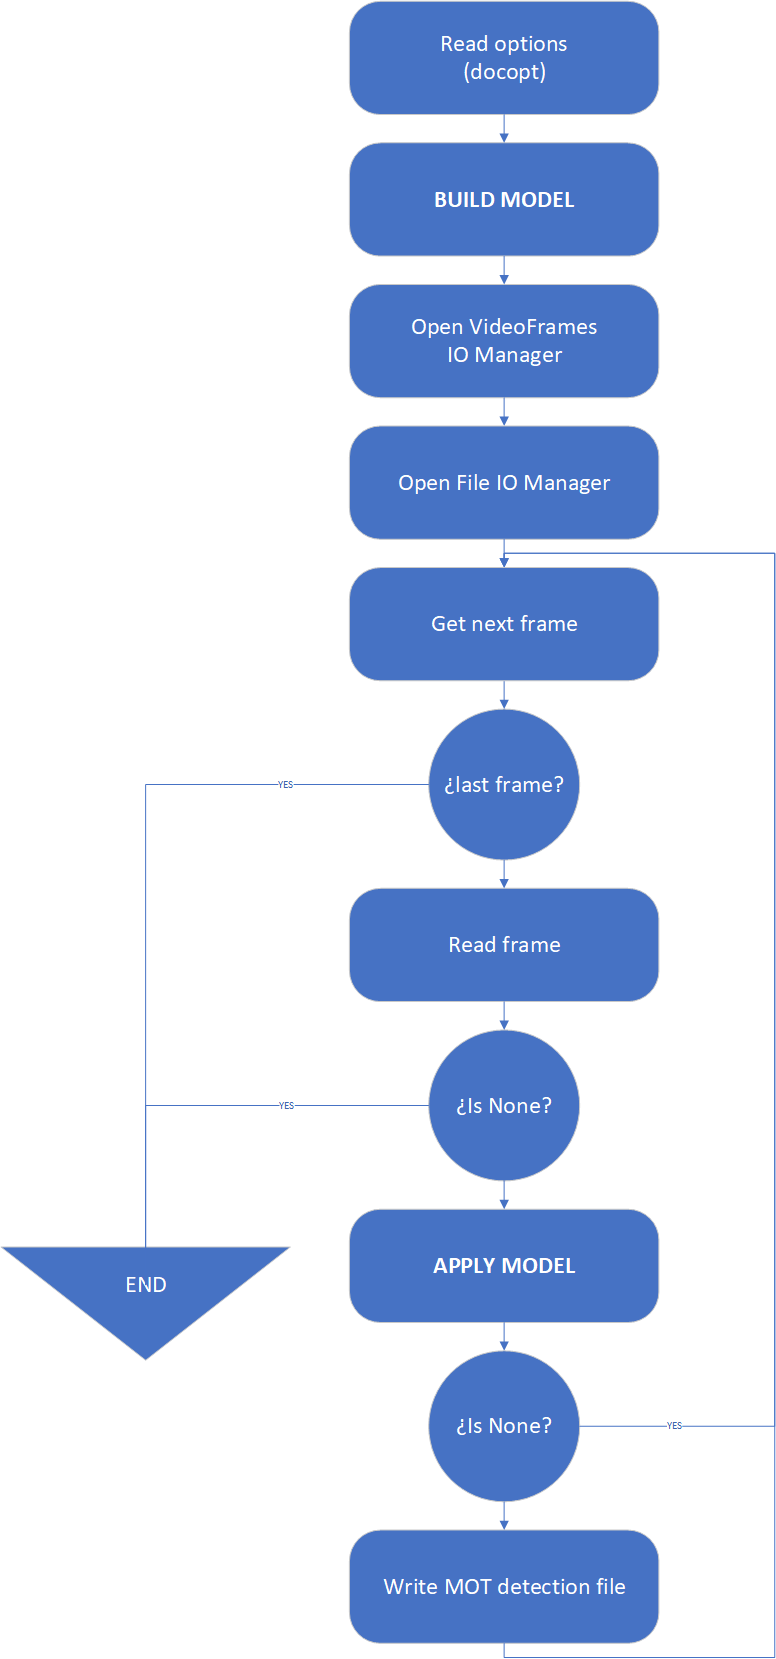
\includegraphics[width=0.6\linewidth]{figures/05_methodology/DetectionScript.png}
%    \caption[Generic detection script]{\footnotesize{
%            Block diagram of the detection script.
%        }}
%    \label{fig:DetectionScript}
%\end{figure}

{
    Initially, there was no labeled data to train any data-driven model, for this reason, the first implemented model was a deductive model.
}

{
    This deductive model, as the examples from the tracking software subsection of the state of the art, is based on background extraction.
}

{
    To ensure accurate background estimation, this model requires a set of training frames. 
    The estimation is performed using a Gaussian Mixture-based model, which becomes reliable after proper training. 
    In this project, 500 frames were used because the input videos allowed it, however, with 50 frames is enough.
}

{
    Once the background is estimated, it is subtracted from the frame to isolate the foreground. 
    A morphological filter consisting in a 5x5 closure to reduce noise inside the ant body, 
    followed by a 3x3 opening is then applied to the foreground to reduce noise in the background estiamtion. 
    The remaining connected components with a minimum pixel count are identified as the output detections.
}

%\begin{figure}[!h]
%    \centering
%    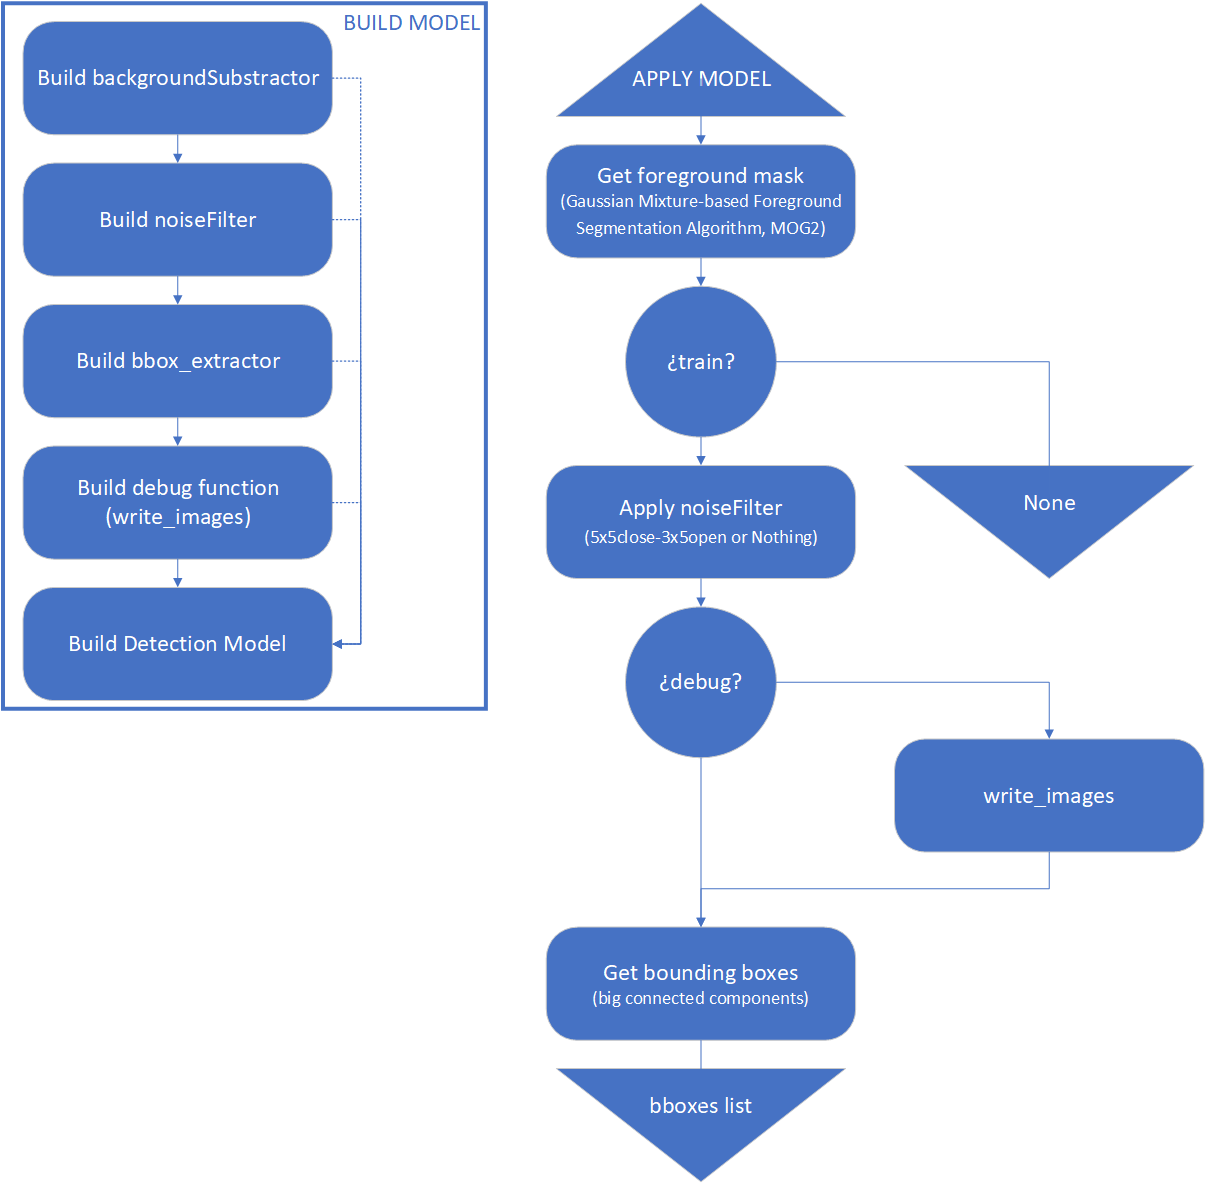
\includegraphics[width=0.6\linewidth]{figures/05_methodology/fgbg_code.png}
%    \caption[Background extraction detection model block diagram]{\footnotesize{
%            Block diagram of the background extraction based model.
%        }}
%    \label{fig:fgbg_code}
%\end{figure}

\FloatBarrier

{
    With the first detection model results, filtered by a tracker and corrected with the developed annotation tools, a initial dataset was created; it was used to train a deep learning model.
    After some iterations of training, detection of new data and cleaning, the final dataset used for detection training was created. 
    The test was performed on an unseen set of data manually annotated: a video fragment which can represent the final deployment.
    The first video was excluded.
}

{
    The following table contains the training, validation and test splits:
}

\begin{table}[H]
    \centering
    \caption[Detection dataset size]{ \footnotesize Detection dataset size.}
    \label{tab:detection splits}

    \begin{tabular}{p{3cm} rr}
        \toprule
        \textbf{Subset} & \textbf{Images} & \textbf{Percentage} \\
        \midrule
        \midrule
        \textbf{Training} & 8374 & 68.7\% \\
        \textbf{validation} & 3662 & 30.1\% \\
        \textbf{Test} & 150 & 1.2\% \\
        \bottomrule
    \end{tabular}
\end{table}

{
    The deep learning model selected for this project is the Ultralytics\cite{Jocher_YOLO_by_Ultralytics_2023} library \ac{YOLOv8} architecture \ac{YOLOv8n} model (detailed in the state of the art section).
    The decision to opt for this architecture was based on state of the art performance in popular challenges as well as simplicity of training and inference deploying (Ultralytics implements most of the standard training features).
}

{
    The choice of model was based on the current problem, the ants on the frames are small objects, and it has two main consequences: 
}

\begin{itemize}
    \item Deep neural networks tend to reduce the spatial dimension while expanding the feature dimension; this means that the ant location becomes uncertain.
    \item Deep neural networks requires a fixed input size, if the input is large, the training may suffer from lack of memory; however, if the input is resized into a smaller size, the small ants may disappear.
\end{itemize}

{
    A slicing windows analysis was deployed in order to solve this issues.
    For the training, 640x640 px crops were used; and, for the inference, a slicing windows was applied using the \ac{SAHI} library\cite{Akyon_Slicing_Aided_Hyper_2022,obss2021sahi}. 
    This method divides the image into a set of overlapped sub-images without any reshaping. 
    However, it results in longer training and inference times, as each image is transformed into multiple sub-images.
}

{
    Additionally, \ac{YOLOv8n}, the smallest \ac{YOLOv8} model, was selected by experimentation.
}

\needspace{0.2\textheight}

\subsubsection{YOLOv8 Training}

{
    Ultralytics is fully integrated with \ac{WandB}\cite{wandb}, a machine learning development platform that helps in the real-time tracking and visualization of experiments, it also have an automatized launcher for hyperparameter sweeping. 
    Using \ac{WandB} resources to visualize enough trainings, the lower and upper thresholds of each available hyperparameter were adjusted until the setting in Table \ref{tab:detection hyperparameters}.
}

\begin{table}[H]
    \centering
    \caption[Detection Model hyperparameters]{ \footnotesize Detection Model hyperparameters.}
    \label{tab:detection hyperparameters}

    \begin{tabularx}{0.9\textwidth}{
        @{\hspace{0.025\textwidth}}
        >{\raggedright\arraybackslash}X
        >{\raggedleft\arraybackslash}X
        @{\hspace{0.025\textwidth}}
    }
        \toprule
        \textbf{Hyperparameter Name} & \textbf{Values} \\
        \midrule
        \midrule
        Hue (maximum deviation) & min=0, max=0.3\\
        Saturation (maximum deviation) & min=0, max=0.5\\
        Value (maximum deviation) & min=0, max=0.5\\
        Rotation (maximum degrees) & min=60º, max=180º\\
        Translation (fraction of input) & min=0, max=0.5\\
        Scale (maximum gain and loss) & min=0, max=1\\
        Flip upside down (probability) & min=0, max=0.5\\
        Flip left-right (probability) & min=0, max=0.5\\
        Mosaic (probability) & min=0, max=1\\
        Shear (maximum degrees) & min=0, max=15\\
        Perspective (fraction) & min=0, max=0.001\\
        Mixup (probability) & min=0, max=0.12\\
        Copy paste (probability) & min=0, max=1\\
        \midrule
        Dropout & \{0, 0.25, 0.5, 0.75\} \\
        \midrule
        Batch size & min=50, max=100 \\
        Optimizer & \{SGD, AdaM\} \\
        Initial learning rate & min=0.001, max=0.01 \\
        Final learning rate & min=0.0001, max=0.001 \\
        Warmup epochs & 10 \\
        Cosine learning rate & \{True, False\} \\
        Momentum & min=0.9, max=0.974 \\
        \midrule
        Maximum epochs & 500 \\
        Early stopping patience & 50 epochs \\
        \midrule
        NMS & \{Agnostic, False\}\\
        NMS IoU & min=0.5, max=1\\
        \bottomrule
    \end{tabularx}
\end{table}

%\needspace{0.25\textheight}

{
    The first group of hyperparameters refer to the data augmentation used to help the model generalize better with the same amount of data, as each time a imaged is loaded, it will be randomly modified within a certain limits. 
    It includes modification in the images coloration, the appearance of the objects within the image, small modifications of the objects (a flip will create a symmetrical but inexistent ant) and some combination of various images. 
    Figure \ref{fig:detector_data_augmentated} shows a set of 16 images after data augmentation.
}

\begin{figure}[!tp]
    \centering
    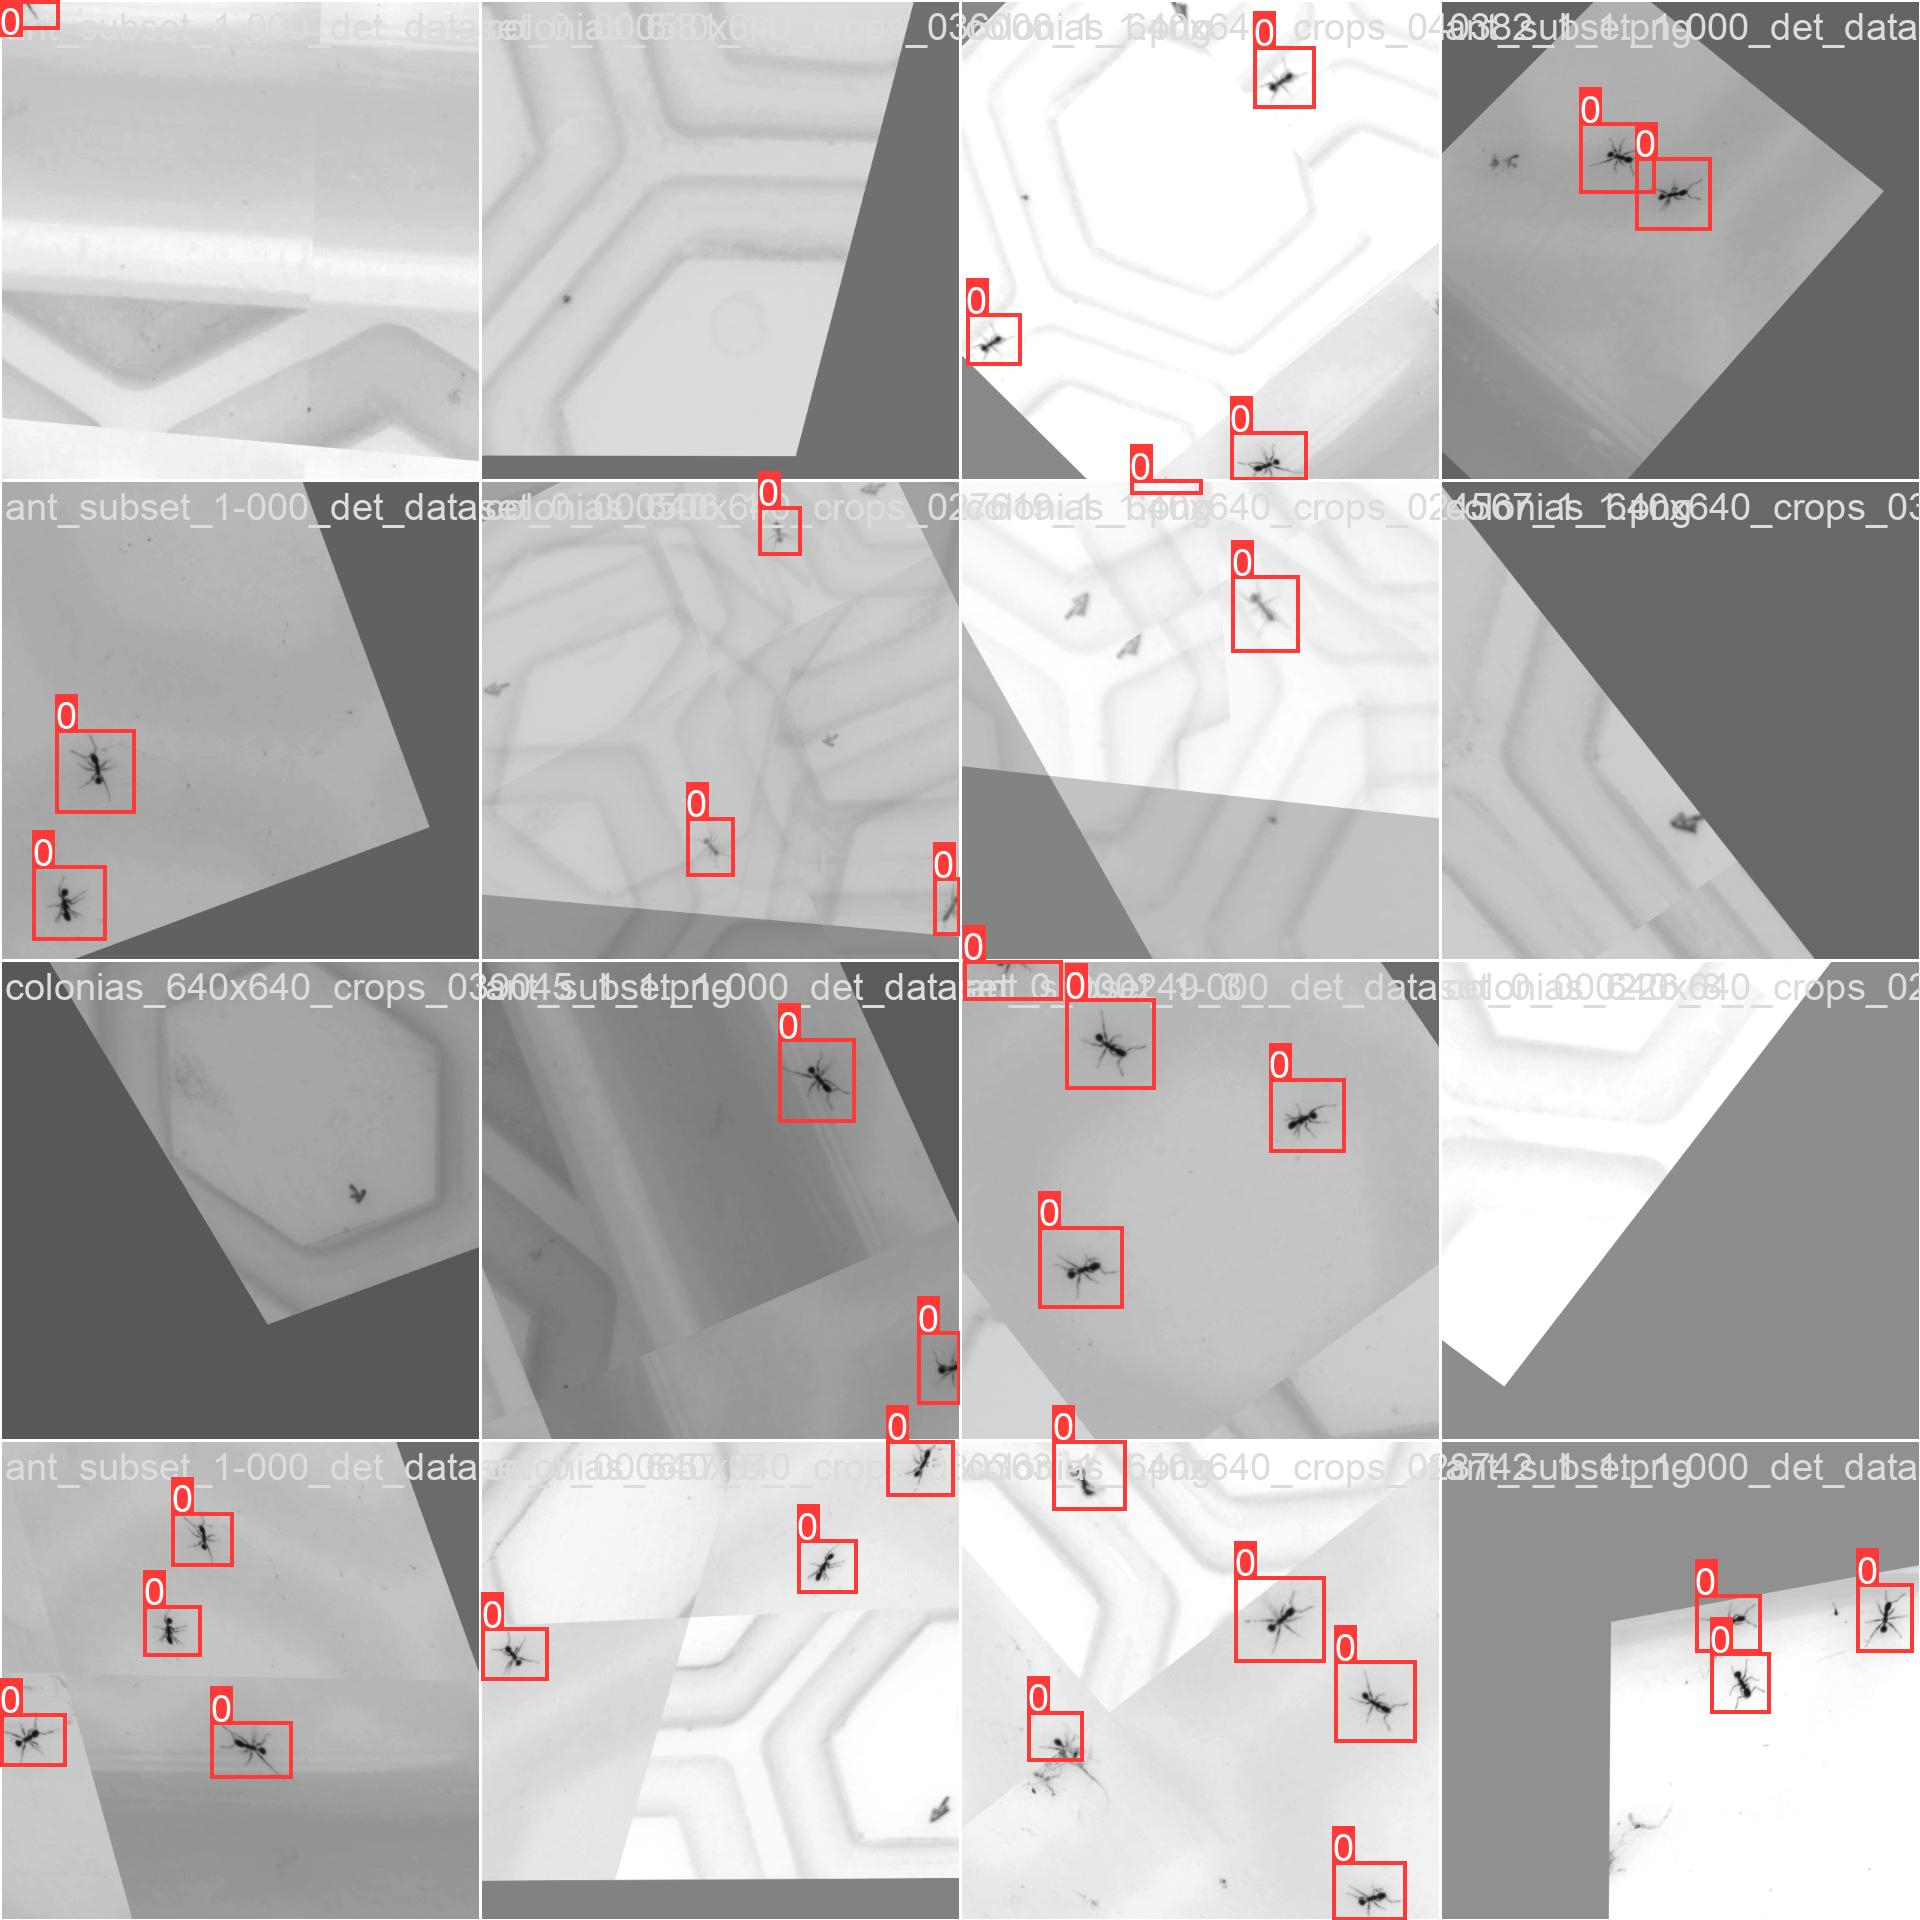
\includegraphics[width=0.5\textwidth]{figures/05_methodology/TrainDataDetector.jpg}
    \caption[YOLOv8 data augmentated]{\footnotesize{Samples of the augmentated training data for the best detector trained.}}
    \label{fig:detector_data_augmentated}
\end{figure}

{
    The second group of hyperparameters refer to the model, in this case, there is only the dropout; it randomly set to zero certain values in the mathematical expression of a forward pass to reduce the number of useless nodes as well as generalize by randomizing.
}

{
    The third group of hyperparameters refer to the weight upgrading to reach an optimum result on the loss function.
    The loss function for these trainings is a combination of binary cross entropy and focal loss for classification (with only one class, ant, both of them are equivalent) and a mean squared error (\ac{MSE}) for the object location.
    The hyperparameters include the number of images used as a representative sample of the world that the model should learn, how the model will find the best weights to fit the current batch samples and the speed (with not a well-defined meaning) at which it will try to reach that weights.
}

{
    The fourth group set a limit on how long it should take to reach the limit, and the maximum steps admissible without validation improvement.
}

{
    The last group is about post-processing the outputs, only the suppression of highly overlapped detections is contemplated.
}

{
    At the end, the best models were selected, added to the detection script with \ac{SAHI} and their outputs were used in the tracker.
}
